\documentclass[11pt]{article}
\usepackage[english]{babel}
\usepackage[utf8x]{inputenc}
\usepackage{amsmath}
\usepackage{graphicx}
\usepackage[colorinlistoftodos]{todonotes}
\usepackage{enumitem}
\usepackage{listings}
\usepackage{verbatim}
\usepackage{eurosym}
\usepackage[export]{adjustbox}
\usepackage{amssymb}
\usepackage{bussproofs}
\usepackage{amsmath}
\usepackage{tikz}

%----------------------------------------------------------------------------------------
%	COVER START
%----------------------------------------------------------------------------------------
\begin{document}

    \begin{titlepage}

        \newcommand{\HRule}{\rule{\linewidth}{0.5mm}}
        \newcommand{\department}{Math Department}
        \newcommand{\course}{Euclidean Geometry}
        \newcommand{\titleValue}{Chronicals}
        \newcommand{\subtitleValue}{Plane-Separation Postulate}
        \newcommand{\authorName}{Alexander Mendozaf}

        \center

        %----------------------------------------------------------------------------------------
        %	HEADER
        %----------------------------------------------------------------------------------------

        \vspace{0.5cm}
        \textsc{\Large \department}\\[0.5cm]
        \textsc{\Large \course}\\[0.5cm]
        \vfill

        %----------------------------------------------------------------------------------------
        %	TITLE
        %----------------------------------------------------------------------------------------

        \HRule\\
        \Huge
        \textbf{\titleValue}\\[0.5cm]
        \Large
        \textbf{\subtitleValue}\\
        \HRule\\[0.5cm]

        %----------------------------------------------------------------------------------------
        %	AUTHOR AND DATE
        %----------------------------------------------------------------------------------------

        \vfill
        \Large
        \textit{\authorName}\\
        {\large \today}\\[2cm]

    \end{titlepage}
%----------------------------------------------------------------------------------------
%	COVER END
%----------------------------------------------------------------------------------------
\section{Plane-Separation Postulate}
    So far we have defined two sets of postulates/axioms, the axioms of incidence and the ruler postulate. Now we are going to define a third one, the \textit{Plane-Separation Postualte}. This postulate states the following:\\

    Let $\alpha$ beff a plane and $l$ a line contained within $\alpha$. There exist two subsets of $\alpha$, $H_1$ and $H_2$ such that:
    \begin{itemize}
        \item $\alpha - l = H_1 \cup H_2$.
        \item $H_1$ and $H_2$ are convex sets.
        \item If $A \in H_1$ and $B \in H_2$, then $\overline{AB} \cap l \not = \emptyset$.
    \end{itemize}
    \begin{center}
        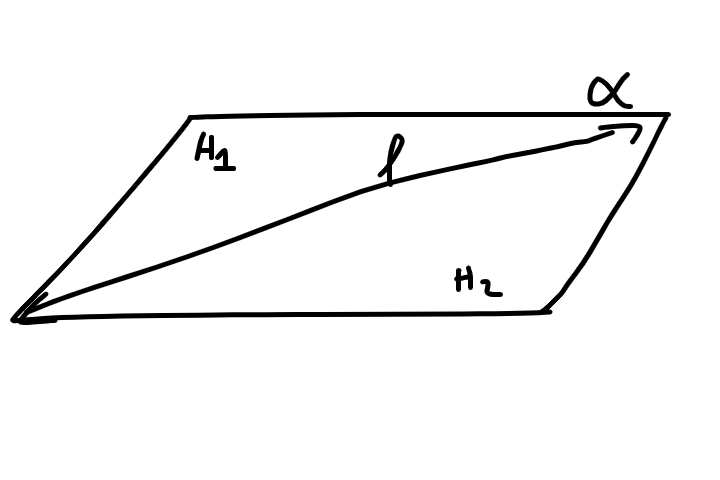
\includegraphics[scale=0.2]{image1.png}
    \end{center}
    Remember that in general a set $\mathcal{A}$ which contains points is said to be convex if and only if for each pair of points $P$ and $Q$ of $\mathcal{A}$, $\overline{PQ} \subseteq \mathcal{A}$.
    Also remember that if the first part of the third item of the list is false, the whole proposition is true. This for definition of implication.

    Now that we have a defined the Plane-Separation Postulate, let's make and prove some basic questions.

    \subsection{Can $H_1$ and $H_2$ be empty?}
        The answer in our current context is no. \textit{Proof}. Let $\alpha$ be a plane and $l$ be a line lying in $\alpha$, then $l$ separates $\alpha$ in two halves $H_1$ and $H_2$, this by the plane-separation postulate.\\

        Now we are going to prove that $H_1$ cannot be empty nor contain a single element. We know that there exist two points $A, B \in l$ and a third point $C$ such that $C \in \alpha$ and is non-collinear to $A$ and $B$, this by the axioms of incidence. Without losing generality, let that point $C$ lie on $H_1$. Now, once again by the axioms of incidence, $\overleftrightarrow{CB}$ exists.\\
        Thus, there exists a point $D$ such that $ C - D - C$ and $D \in H_1$. If $D \not \in H_1$ then either $D \in l$ or $D \in H_2$. Let us observe what happens in both cases.\\

        When $D \in l$. We know that $l \cap \overleftrightarrow{BC} = \{C\}$ this by the theorem of intersection of two lines. Then by definition of intersection, $D \in l \cap \overleftrightarrow{BC}$, thus $D = C$. This is a contradiction because is given that $C - D -C$ and by definition $D \not = C$.

        When $D \in H_2$.
\end{document}